
% ************* PREAMBLE

\documentclass{beamer}

% ------------- THEME

\usetheme[block=fill]{metropolis}
\usepackage{appendixnumberbeamer}
\usepackage{booktabs}
\usepackage[scale=2]{ccicons}
\usepackage{pgfplots}
\usepgfplotslibrary{dateplot}
\usepackage{xspace}
\newcommand{\themename}{\textbf{\textsc{metropolis}}\xspace}

% ------------- REFERENCES

\usepackage[backend=biber,style=apa]{biblatex}
\addbibresource{references.bib}

% ------------- COLOR

\usepackage{xcolor}
\definecolor{lightgray}{RGB}{211, 211, 211}

% ------------- OTHER PACKAGES

\usepackage[italian]{babel}
\usepackage[utf8]{inputenc}

\usepackage{stmaryrd}

\usepackage{amssymb}
\usepackage{amsmath}
\usepackage{latexsym}
\usepackage{amsthm}
\usepackage{mathabx}

\usepackage{hyperref}
\usepackage{caption}

% ------------- GENERAL INFORMATION

\title{Towards a Categorical Foundation of Deep Learning: A Survey}
\subtitle{Una rassegna di approcci categorici al \textit{deep learning}}
\author{Francesco Riccardo Crescenzi\\Relatore: Fabio Zanasi}
\institute{Alma mater studiorum - Università di Bologna \\ CdL in Matematica}


% ************* DOCUMENT

\begin{document}

\maketitle

\begin{frame}[standout]
    \Huge We are in an AI summer, but is winter coming?
\end{frame}
\begin{frame}{Problemi con il deep learning}
    \large Mancano fondamenta teoriche:
    \begin{itemize}
        \item<1-> \textbf{design ad hoc} {\footnotesize(\cite{gavranovic2024fundamental})}
        \item<2-> \textbf{complessità fine a se stessa} {\footnotesize(\cite{rahimi2017machine})}
        \item<3-> \textbf{fragilità} {\footnotesize(\cite{gavranovic2024fundamental})}
    \end{itemize}
\end{frame}

\begin{frame}{Problemi con il deep learning}
    \large La ricerca viene rallentata da:
    \begin{itemize}
        \item<1-> \textbf{research debt} {\footnotesize(\cite{olah2017research})}
        \item<2-> \textbf{mancata replicabilità} {\footnotesize(\cite{raff2019step})}
    \end{itemize}
\end{frame}

\begin{frame}[standout]
    \centering \Huge Teoria delle categorie: \\\large una lingua franca della matematica e delle scienze
\end{frame}

\begin{frame}{Teoria delle categorie applicata}
    \centering La teoria delle categorie studia strutture e relazioni, e può essere vista come un'estensione del celebre \textit{Erlangen Programme}.

    \centering La teoria delle categorie può essere applicata con successo anche in fisica, informatica, chimica... ovunque ci sia \textbf{composizionalità} (\cite{fong2018seven}).
\end{frame}

\begin{frame}{Teoria delle categorie applicata}
    \begin{itemize}
        \item<1-> \textbf{lenti parametriche} {\footnotesize (\cite{gavranovic2024fundamental}, \cite{cruttwell2022categorical})}
        \item<2-> \textbf{categorical deep learning}{ \footnotesize(\cite{gavranovicposition})}
        \item<3-> \textbf{integral transforms} {\footnotesize(\cite{dudzik2022graph}, \cite{dudzik2024asynchronous})}
        \item<4-> \textbf{functor learning} {\footnotesize(\cite{gavranovic2019compositional}, \cite{sheshmani2021categorical}, \cite{chytas2024poolingimagedatasetsmultiple})}
        \item<5-> \textbf{compositional distributional model of meaning} {\footnotesize(\cite{clark2007combining}, \cite{coecke2010mathematical}, \cite{lewis2019compositionality})}
        \item<6-> \textbf{neural circuit diagrams} {\footnotesize(\cite{abbott2023robust})}
        \item<7-> \textbf{string diagrams with universal approximators} {\footnotesize(\cite{khatri2024anatomy})}
    \end{itemize}
\end{frame}

\begin{frame}{Teoria delle categorie applicata}
    \begin{itemize}
        \item \textbf{lenti parametriche} {\footnotesize (\cite{gavranovic2024fundamental}, \cite{cruttwell2022categorical})}
        \item \textbf{categorical deep learning}{ \footnotesize(\cite{gavranovicposition})}
        \item \textcolor{lightgray}{\textbf{integral transforms} {\footnotesize(\cite{dudzik2022graph}, \cite{dudzik2024asynchronous})}}
        \item \textcolor{lightgray}{\textbf{functor learning} {\footnotesize(\cite{gavranovic2019compositional}, \cite{sheshmani2021categorical}, \cite{chytas2024poolingimagedatasetsmultiple})}}
        \item \textcolor{lightgray}{\textbf{compositional distributional model of meaning} {\footnotesize(\cite{clark2007combining}, \cite{coecke2010mathematical}, \cite{lewis2019compositionality})}}
        \item \textcolor{lightgray}{\textbf{neural circuit diagrams} {\footnotesize(\cite{abbott2023robust})}}
        \item \textcolor{lightgray}{\textbf{string diagrams with universal approximators} {\footnotesize(\cite{khatri2024anatomy})}}
    \end{itemize}
\end{frame}

\begin{frame}[standout]
    \huge Lenti parametriche \\\large per modellare il gradient-based learning
\end{frame}

\begin{frame}{Gradient-based learning con lenti parametriche}
    Il gradient-based learning segue tre principi fondamentali:
    \begin{itemize}
        \item<1-> \textbf{parametricità}
        \item<2-> \textbf{bidirezionalità}
        \item<3-> \textbf{differenziabilità}
    \end{itemize}
\end{frame}

\begin{frame}{Gradient-based learning con lenti parametriche}
    \begin{block}{DEFINIZIONE: Il costrutto $\mathbf{Para}$}
        Sia $(\mathcal{C},I,\otimes)$ una categoria monoidale strettamente simmetrica. Allora, $\mathbf{Para}_{\otimes}(\mathcal{C})$ è la $2$-categoria definita come segue.
        \begin{itemize}
          \item Le $0$-celle sono oggetti di $\mathcal{C}$.
          \item Le $1$-cells sono coppie $(P,f): A \to B$, dove $P : \mathcal{C}$ e $f: P \otimes A \to B$.
          \item The $2$-celle sono $r: (P,f) \Rightarrow (Q,g)$, dove $r: P \to Q$ è un morfismo in $\mathcal{C}$ che rispetta certe condizioni di naturalità.
        \end{itemize}
        Vedasi \cite{gavranovic2024fundamental}.
      \end{block}
\end{frame}

\begin{frame}{Gradient-based learning con lenti parametriche}
    \begin{figure}
        \begin{center}
            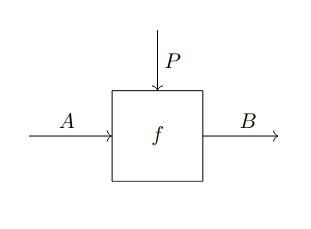
\includegraphics[width=0.5\textwidth]{figures/para.png}
            \caption*{\cite{gavranovic2024fundamental}}
        \end{center}
    \end{figure}
\end{frame}

\begin{frame}{Gradient-based learning con lenti parametriche}
    \begin{figure}
        \begin{center}
            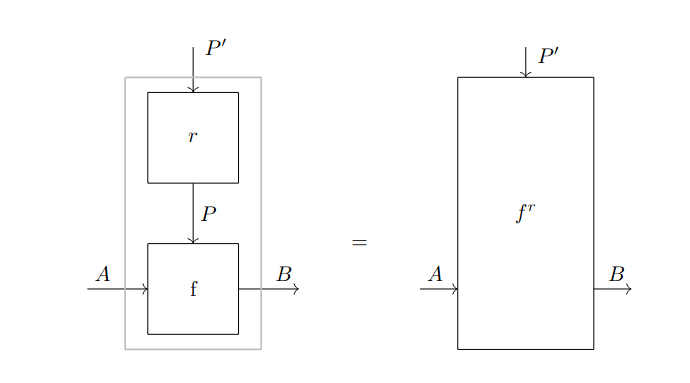
\includegraphics[width=0.7\textwidth]{figures/para_reparametrization.png}
            \caption*{\cite{gavranovic2024fundamental}}
        \end{center}
    \end{figure}
\end{frame}

\begin{frame}{Gradient-based learning con lenti parametriche}
    \begin{figure}
        \begin{center}
            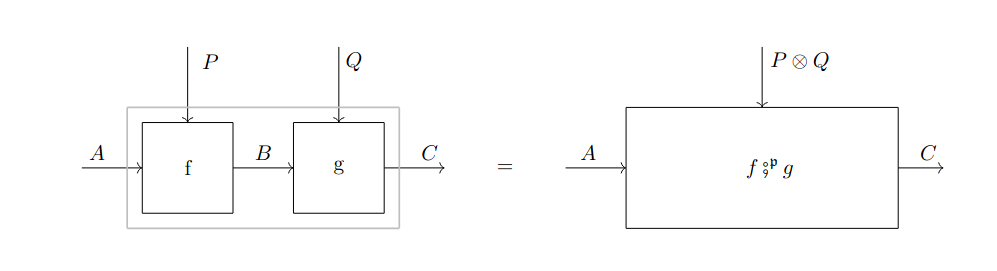
\includegraphics[width=\textwidth]{figures/para_composition.png}
            \caption*{\cite{gavranovic2024fundamental}}
        \end{center}
    \end{figure}
\end{frame}

\begin{frame}{Gradient-based learning con lenti parametriche}
    \begin{block}{DEFINIZIONE: Il costrutto $\mathbf{Lens}$}
        Sia $(\mathcal{C},1,\times)$ una categoria Cartesiana. Allora, $\mathbf{Lens}(\mathcal{C})$ è la categoria definita come segue.
        \begin{itemize}
          \item Un oggetto di $\mathbf{Lens}(\mathcal{C})$ è una coppia $\left(\begin{smallmatrix} A \\ A' \end{smallmatrix}\right)$ di oggetti di $\mathcal{C}$.
          
          \item Un morfismo $\left(\begin{smallmatrix} A \\ A' \end{smallmatrix}\right) \to \left(\begin{smallmatrix} B \\ B' \end{smallmatrix}\right)$ (anche chiamato lente) è una coppia $\left(\begin{smallmatrix} f \\ f' \end{smallmatrix}\right)$ di morfismi di $\mathcal{C}$ tali che $f: A \to B$ and $f': A \times B' \to A'$. La mappa $f$ è nota come \textit{forward pass} della lente, mentre la mappa $f'$ è nota come \textit{backward pass}.
        \end{itemize}
        Vedasi \cite{cruttwell2022categorical}.
      \end{block}
\end{frame}

\begin{frame}{Gradient-based learning con lenti parametriche}
    \begin{figure}
        \begin{center}
            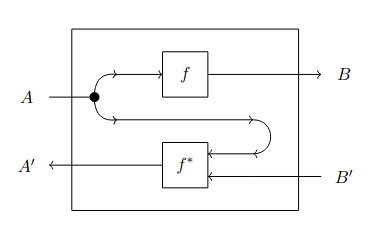
\includegraphics[width=0.7\textwidth]{figures/lens_inner_view.png}
            \caption*{\cite{cruttwell2022categorical}}
        \end{center}
    \end{figure}
\end{frame}

\begin{frame}{Gradient-based learning con lenti parametriche}
    \begin{figure}
        \begin{center}
            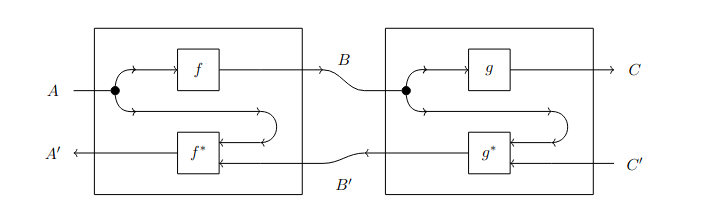
\includegraphics[width=\textwidth]{figures/lens_composition.png}
            \caption*{\cite{cruttwell2022categorical}}
        \end{center}
    \end{figure}
\end{frame}

\begin{frame}{Gradient-based learning con lenti parametriche}
    \begin{block}{DEFINIZIONE: Cartesian reverse differential category}
        Una \textit{Cartesian reverse differential category} (CRDC) $\mathcal{C}$ è una categoria Cartesiana con una struttura additiva dove è definito un operatore differenziale $\mathrm{R}$ che ha le proprietà di una \textit{reverse derivative}.
        Si vedano \cite{cockett2019reverse} e \cite{gavranovic2024fundamental}.
      \end{block}

      \begin{block}{ESEMPIO: $\mathbf{Smooth}$}
        Consideriamo $\mathbf{Smooth}$, ovvero la categoria degli spazi Euclidei e delle funzioni liscie. $\mathbf{Smooth}$ è una CRDC rispetto all'operatore
        \[\mathrm{R}[f]: (x,y) \mapsto \mathcal{J}_f(x)^Ty.\]
      \end{block}
\end{frame}

\begin{frame}{Gradient-based learning con lenti parametriche}
    \begin{block}{TEOREMA: Lenti parametriche con backward pass additivo}
        Sia $\mathcal{C}$ una CRDC. Consideriamo la sottocategoria $\mathbf{Lens}_A(\mathcal{C})$ di $\mathbf{Lens}(\mathcal{C})$ costuituita da lenti nella forma $\left(\begin{smallmatrix} f \\ \mathrm{R}[f]\end{smallmatrix}\right)$. È possibile applicare il costrutto $\mathbf{Para}$ a $\mathbf{Lens}_A(\mathcal{C})$.
    \end{block}   

    $\mathbf{Para}_{\otimes}(\mathbf{Lens}_A(\mathcal{C}))$ è una categoria di lenti parametriche il cui \textit{backward pass} contiene informazioni necessarie e sufficienti per implementare la \textit{backpropagation}.
\end{frame}

\begin{frame}{Gradient-based learning con lenti parametriche}
    \begin{figure}
        \begin{center}
            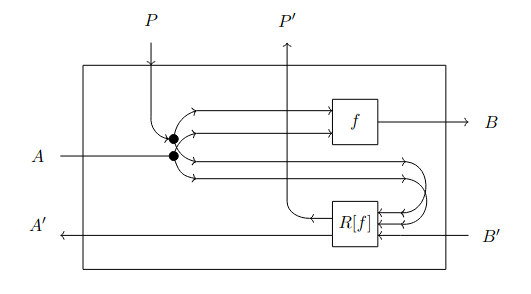
\includegraphics[width=\textwidth]{figures/parametric_lens.png}
            \caption*{\cite{cruttwell2022categorical}}
        \end{center}
    \end{figure}
\end{frame}

\begin{frame}{Gradient-based learning con lenti parametriche}
    \begin{figure}
        \begin{center}
            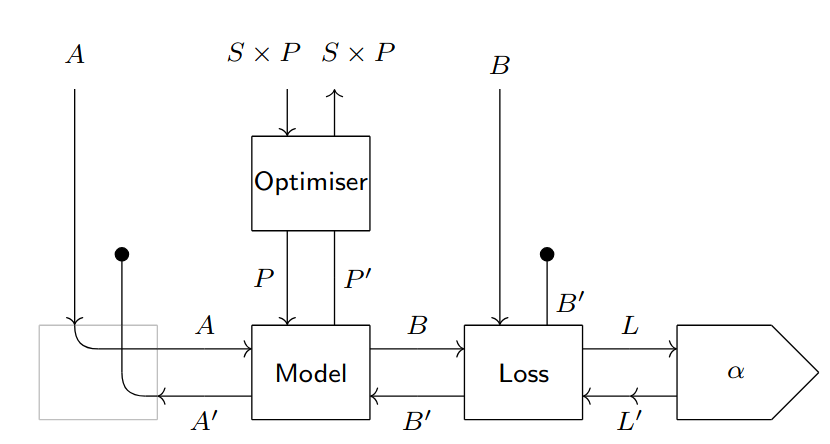
\includegraphics[width=\textwidth]{figures/lenses_supervised_learning2.png}
            \caption*{\cite{cruttwell2022categorical}}
        \end{center}
    \end{figure}
\end{frame}

\begin{frame}[standout]
    \huge Categorical deep learning: \\\large (co)algebre categoriche \\come teoria delle architetture
\end{frame}

\begin{frame}{Categorical deep learning}
    \begin{block}{\textit{Geometric deep learning}}
        Il \textit{geometric deep learning} è una teoria delle architetture di reti neurali che imita l'\textit{Erlangen Programme}, organizzando le architetture in base al concetto di equivarianza rispetto ad azioni di gruppi (\cite{bronstein2021geometric}).
    \end{block}
\end{frame}

\begin{frame}{Categorical deep learning}
    \begin{block}{DEFINIZIONE: Funzione equivariante}
        Sia $G$ be un gruppo e siano $(S, \cdot)$ e $(T, \ast)$ azioni di $G$. Una funzione $f: S \to T$ è equivariante rispetto a tali azioni se 
        \[f(g \cdot s) = g \ast f(s),\] 
        per ogni $s \in \mathcal{S}$ e per ogni $g \in \mathcal{G}$.
    \end{block}

    \begin{block}{ESEMPIO}
        I \textit{convolutional layers} rappresentano mappe invarianti rispetto a traslazioni.
    \end{block}
\end{frame}

\begin{frame}{Categorical deep learning}
    \begin{block}{\textit{Categorical deep learning}}
        Il \textit{categorical deep learning} è una teoria delle architetture di reti neurali che generalizza il GDL, organizzando le architetture in base al concetto di omomorfismo di (co)algebre categoriche (\cite{gavranovicposition}).
    \end{block}
\end{frame}

\begin{frame}{Categorical deep learning}
    \begin{block}{DEFINIZIONE: Algebra su un endofuntore}
        Sia $F: \mathcal{C} \to \mathcal{C}$ un endofuntore. Un'algebra su $F$ è una coppia $(A,a)$ dove $A$ è un oggetto di $\mathcal{C}$ e $a: F(A) \to A$ è un morfismo in $\mathcal{C}$.
    \end{block}

    \begin{block}{DEFINIZIONE: Omomorfismo di algebre}
        Siano $(A,a)$ e $(B,b)$ algebre sollo stesso endofuntore $F: \mathcal{C} \to \mathcal{C}$. Un omomorfismo di algebre $(A,a) \to (B,b)$ è un morfismo $f: A \to B$ in $\mathcal{C}$ tale che $F(f) \fatsemi b =  a \fatsemi f$.
    \end{block}
\end{frame}

\begin{frame}{Categorical deep learning}
    \begin{figure}
        \begin{center}
            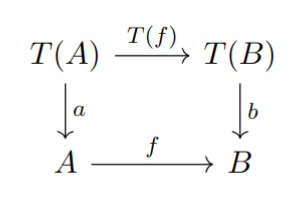
\includegraphics[width=0.5\textwidth]{figures/algebra_hom.png}
            \caption*{}
        \end{center}
    \end{figure}
\end{frame}

\begin{frame}{Categorical deep learning}
    Il \textit{categorical deep learning} getta un ponte tra informatica classica e machine learning identificando architetture neurali come generalizzazioni parametriche di strutture dati note.

    \begin{figure}
        \begin{center}
            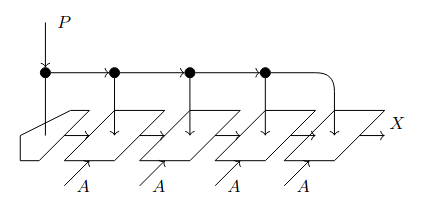
\includegraphics[width=0.7\textwidth]{figures/folding_rnn.png}
            \caption*{\cite{gavranovicposition}}
        \end{center}
    \end{figure}
\end{frame}

\begin{frame}{Categorical deep learning}
    \begin{figure}
        \begin{center}
            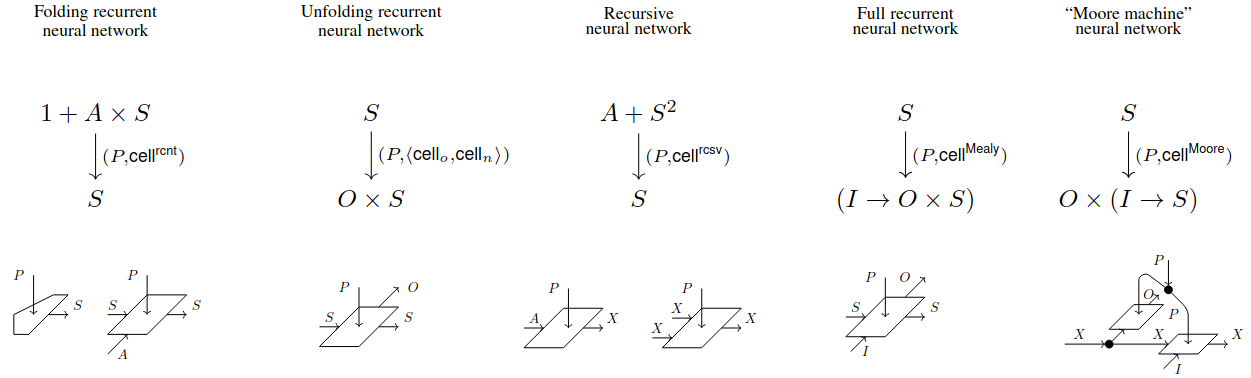
\includegraphics[width=1\textwidth]{figures/cells.png}
            \caption*{\cite{gavranovicposition}}
        \end{center}
    \end{figure}
\end{frame}

\begin{frame}[standout]
    \huge Brevi accenni \\\large agli altri approcci trattati nella tesi
\end{frame}

\begin{frame}{Integral transform}

    \begin{figure}
        \begin{center}
            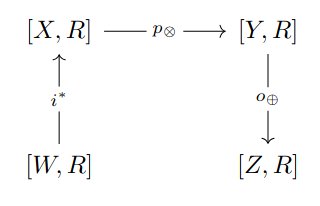
\includegraphics[width=0.5\textwidth]{figures/integral_transform.png}
            \caption*{\cite{dudzik2022graph}}
        \end{center}
    \end{figure}

    L'\textit{integral transform} è un costrutto categorico che agisce come struttura fondamentale condivisa da GNNs e da algoritmi di programmazione dinamica. Individuare questa struttura comune è utile per aumentare l'\textit{algorithmic alignment} (\cite{dudzik2022graph}, \cite{dudzik2024asynchronous}). 
\end{frame}

\begin{frame}{Functor learning}
    Il \textit{functor learning} è un paradigma di machine learning che consiste nell'apprendere un funtore tra categorie invece che un semplice morfismo tra oggetti.

    Apprendere un funtore permette di sfruttare la struttura categorica dei dati per ridurne la complessità e per imporre condizioni di invarianza (\cite{sheshmani2021categorical}, \cite{chytas2024poolingimagedatasetsmultiple}).
\end{frame}

\begin{frame}{Compositional distributional model}
    Il \textit{compositional distributional model of natural language} utilizza il concetto di categoria compatta chiusa per unire un modello simbolico della lingua (\textit{pregroup grammar}) a un modello distribuzionale (\textit{word embedding}), ottenendo i vantaggi di entrambi (\cite{clark2007combining}, \cite{coecke2010mathematical}, \cite{lewis2019compositionality}).

    \begin{figure}
        \begin{center}
            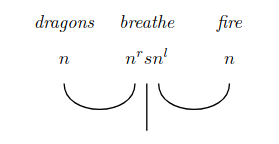
\includegraphics[width=0.5\textwidth]{figures/pregroup1.png}
            \caption*{\cite{lewis2019compositionality}}
        \end{center}
    \end{figure}
\end{frame}

\begin{frame}{Neural circuit diagrams}
    I \textit{neural circuit diagrams} sono diagrammi con semantica categorica utili per rappresentare in modo dettagliato archittetture neurali (\cite{abbott2023robust}).
\end{frame}

\begin{frame}{Neural circuit diagrams}
    \begin{figure}
        \begin{center}
            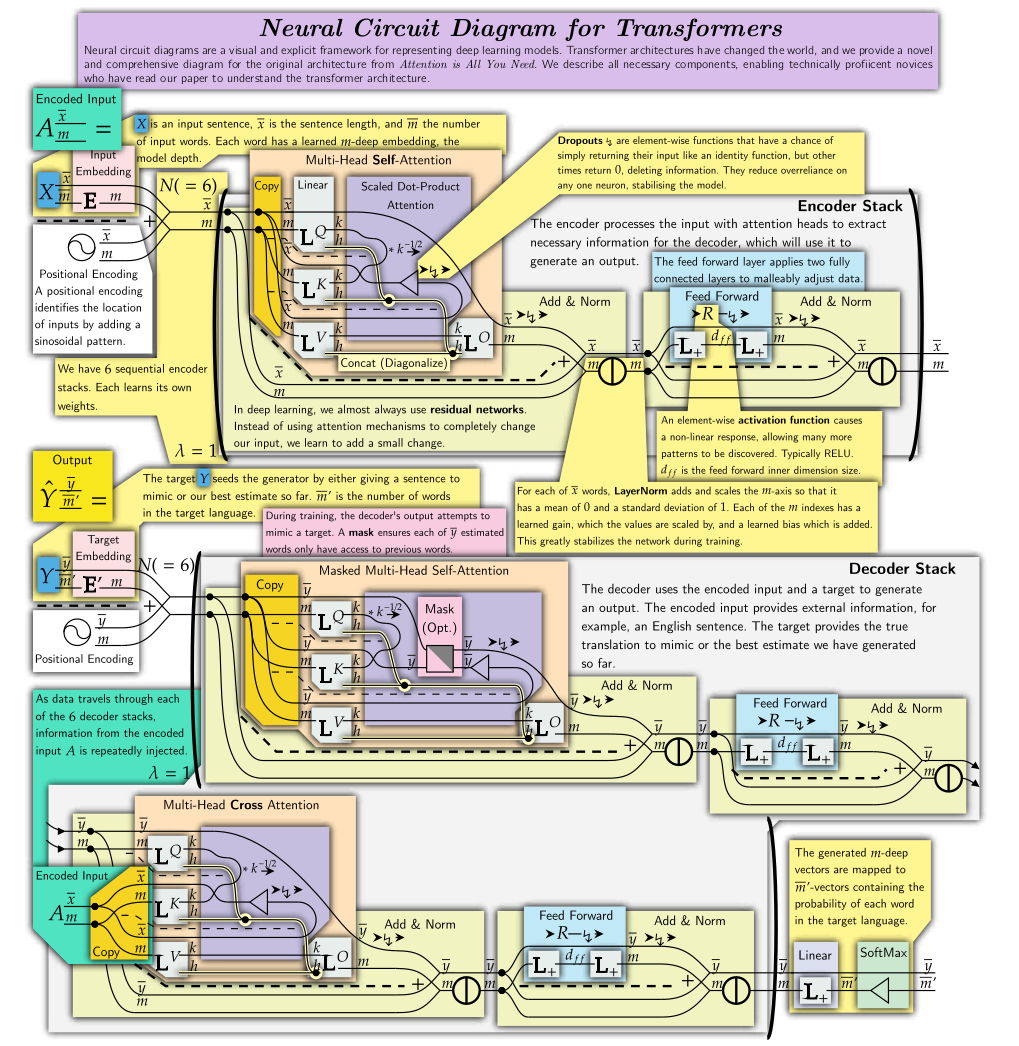
\includegraphics[angle=90,width=1\textwidth]{figures/transformer_ncd.png}
            \caption*{\cite{abbott2023robust}}
        \end{center}
    \end{figure}
\end{frame}

\begin{frame}{String diagrams with universal approximators}
    Gli \textit{string diagrams with universal approximators} sono diagrammi con semantica categorica utili per rappresentare architetture neurali (\cite{khatri2024anatomy}).
    
    A differenza dei \textit{neural circuit diagrams}, gli \textit{string diagrams with universal approximators} usano il concetto di \textit{unversal approximator} per consentire astrazione tramite \textit{rewrite}.
\end{frame}

\begin{frame}{String diagrams with universal approximators}
    \begin{figure}
        \begin{center}
            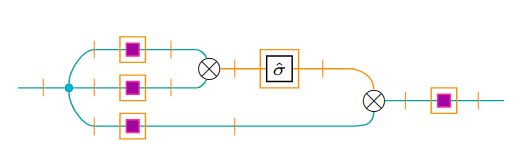
\includegraphics[width=1\textwidth]{figures/khatri_attention.png}
            \caption*{\cite{khatri2024anatomy}}
        \end{center}
    \end{figure}
\end{frame}

\begin{frame}[standout]
    \huge Prospettive future
\end{frame}

\begin{frame}{Prospettive future}
    C'è una competizione in corso tra varie discipline che puntano a spiegare il deep learning utilizzando ciascuna i propri strumenti:
    \begin{itemize}
        \item<1-> \textbf{fisica matematica} {\footnotesize (e.g. \cite{roberts2022principles})},
        \item<2-> \textbf{topologia} {\footnotesize (e.g. \cite{hensel2021survey})},
        \item<3-> \textbf{probabilità} {\footnotesize (e.g. \cite{patel2015probabilistic})},
        \item<4-> e così via...
    \end{itemize}
    
\end{frame}

\begin{frame}{Prospettive future}
    La teoria delle categorie, oltre a offrire strumenti propri, potrebbe creare un ponte tra queste discipline e potrebbe unificare i loro approcci in una teoria generale del deep learning.
\end{frame}

\begin{frame}[allowframebreaks]
    \printbibliography
\end{frame}

\end{document}